\subsection{Representation fairness}\label{subsec:repfair}
%A general discussion about the rationale behind representation fairness, its goals, connection to incentives, highload epochs, etc
Representation fairness is an important and difficult to analyze property of \nameNS. It becomes relevant in high-load epochs, when $etx$ selection is subject to manipulation; and it is strongly linked to the incentive structure the protocol is designed for. As mentioned before, in this article we do not discuss incentives that dictate nodes' decisions and operations. We merely say that nodes are assumed to compete for block space - each node, trying to service its own users as fast as possible - and might use Eblock construction strategies that are not compliant with \nameNS's instructions. We emphasize that such behavior is a clear violation of the protocol rules and is considered Byzantine (thus, at most $f$ nodes might choose to do so).

In such circumstances, representation fairness aims to guarantee that the blockchain is a faithful representation of the nodes' issuance rate (i.e., the relative amount of $etx$s each node produces). This notion is not enough though, as low-load epochs follow high-load ones such that eventually all $etx$s get committed. We therefore add a crucial aspect to representation fairness - the time aspect. We illustrate this by an example, if a node issues $10\%$ of the overall $etx$s, then the percentage of its $etx$s in the blockchain should be, \textbf{at all times}, close to $10\%$, no matter what strategy it follows, or what other nodes do. Moreover, if the size of the global Epool is, say, $5b$, then in average an $etx$ should wait $5$ terms to be committed to the blockchain.

In this section we first describe the model under which the problem is analyzed. We then formulate three basic properties that \name is shown to satisfy. These properties, combined, provide evidence that \name is highly resistant to attacks against representation fairness - both in terms of their ability to create an unfair chain, as well as in waiting time. 

%How we model the problem - general setting and simplifications, what we don't model, distributions, RVs. If we use these vectors rather then RVs explain why it is not critical to the analysis and that it simplifies things. 
%There are two typical types of highload epochs - we focus on one. Why is it enough? 
To state and prove fairness properties, we use the following model for \nameNS's operation and the way new Eblocks are constructed and appended to the blockchain. In order to set a single time-line to distinguish between terms, we make an arbitrary choice and say that term $r$ starts when some correct node reveals $DB^{r-1}$ (it ends when term $r+1$ starts). We first define the mathematical objects which come into play: 

\begin{itemize}
	\item \textbf{Issuance distribution}. The \textit{issuance distribution} $\MBI^r\in \mathbb{R}^n$ is a probability vector (i.e., its coordinates sum to $1$), for which the $j$ coordinate stands for the fraction of $etx$s owned by node $j$ among all $etx$s issued during term $r$. 
    \item \textbf{Global EPool distribution}. The \textit{$GEP$ distribution} $\MBG^r\in \mathbb{R}^n$ is a probability vector for which the $j$ coordinate stands for the fraction of $etx$s in $GEP^r$ owned by node $j$.  
     \item \textbf{Block distribution}. The \textit{block distribution} $\MBB^r\in \mathbb{R}^n$ is a probability vector for which the $j$ coordinate stands for the fraction of $etx$s in $EB^r$ owned by node $j$.
    \item \textbf{Chain distribution}. The \textit{chain distribution} $\MBC^r\in \mathbb{R}^n$ is a probability vector for which the $j$ coordinate stands for the fraction of $etx$s owned by node $j$ which were appended to the blockchain by term $r$. Notice that $\MBC^r=\frac{1}{r}\sum_s \MBB^s$.
\end{itemize}

When we wish to refer to the actual set of $etx$s associated with each distribution vector $\mathbf{V}$, we use calligraphic font $\mathcal{V}$. For example, $\MC{I}^r$ is the set of $etx$s issued during term $r$. We refer to $\vert \MC{I}^r\vert$ as the \textit{issuance rate} of term $r$. Note that the vector $\vert \MC{I}^r\vert\cdot \MBI^r$ is the vector for which the $j$ coordinate stands for the absolute number of $etx$s owned by node $j$, issued during term $r$. Our model assumptions can now be formulated as follows: 
\begin{itemize}
	\item $\MBI^r$ is a fixed vector (not necessarily uniform) for all $r$. We thus denote from now on $\MBI^r=\MBI$.
    \item The issuance rate for all $r$ is $b$, i.e., the number of issued $etx$s during each term is constant, and equals the size of an Eblock. As a consequence, $|GEP^r|$ is fixed for all $r$, and we denote $|GEP^r|=\Gamma\cdot b$ for some fixed $\Gamma\ge 1$.
    \item An Eblock is constructed in such a way that $\MBB^r$ exactly reflects $\MBG^r$, rather than being a random sample of it. For a correct primary, $\MBB^r=\MBG^r$, which illustrates the fact that a correct primary constructs its Epool using our correlated sampling construction, which is assumed to be distributed more or less like $\MBG^r$. For a Byzantine primary $\MBB^r=\beta\cdot \MBG^r +(1-\beta)\cdot \MBG^r_B$, for some probability vector $\MBG^r_B$, that stands for the part of the Eblock which it constructs maliciously. Notice that with this assumption, our model loses the random nature of Eblock construction.
\end{itemize}
We stress that while these simplifications may seem strong and limiting, we believe this model does capture the essential issues related to representation fairness in \nameNS. To (informally) justify this belief, we give short intuition for each of the above assumptions:
\begin{itemize}
	\item \textbf{Fixed issuance rate and fixed $\pmb{GEP}$ size.} In high-load epochs Epools are large, but cannot be too large. Otherwise, $etx$s wait too long to be appended to the blockchain and the system is de-facto broken. If the issuance rate is larger than the appending rate per term, it will not take long before the global Epool is too big for the system to handle. Hence, the relevant situation to consider is a stable state where Epools are of a roughly fixed size $\Gamma\cdot b$, moderately larger than $b$ (typically, $1\leq \Gamma\leq 20$). Hence the number of issued $etx$s per term should be, on average, $b$, and not much is lost assuming it is exactly $b$.
    \item \textbf{Fixed issuance distribution.} We cannot expect \name to guarantee complete fairness towards an issuance distribution which changes very rapidly - and in fact, it makes no sense to do so. The right property to ask for is fairness towards an \textit{accumulative} issuance distribution (say of the last $20$ terms). Over time, we can expect to see a more stable accumulative issuance distribution (which can change in the next chunk of $20$ terms), and expect the $GEP$ distribution to represent it faithfully. This motivates our assumption of a fixed issuance distribution. Moreover, our proof in fact shows how long it actually takes for the $GEP$ distribution to represent the issuance distribution faithfully, once the latter changed from one stable distribution to another. %\red{add recovery time and rephrase a bit}.
    \item \textbf{Fixed Eblock distribution.} This is our most serious assumption, and the only one we expect to result in a slight difference between the theoretical analysis and the real time performance of the system. Nevertheless, when $b$ is large enough, and on the other hand $\Gamma$ is not too large, it is reasonable to expect that a legally constructed $EB$ will be distributed more or less like $GEP$, and even more so if we average over several such Eblocks.
%need to rephrase and relax the first sentence a bit.
\end{itemize}

% Our investigation begins at time $t_0$ and term number $r$. We assume fixed issuance rate throughout the scope of the analysis, where in each term a certain amount of $etx$s is injected into the network (according to the issuance rate), and $b$ $etx$s are added to the blockchain by the elected primary. The primary is either Byzantine, with probability $\frac{f}{n}$, or correct, with probability $1- \frac{f}{n}$. Correct Eblocks are constructed according to the protocol's rules, while Byzantine ones deviate by the maximal amount of $etxs$ that still enables their Eblocks to be committed (i.e., $(1-\beta)b$). In this regard, our analysis is a worst-case analysis rather then an average-case one. Finally, in order to set a single time-line, we make a rather arbitrary choice - term $r$ starts when some correct node reveals $DB^{r-1}$.

% \noindent \textbf{Model for simulations}
% \begin{itemize}
% \item The issuance rate, $\mathbf{I}$, is a constant vector with $n$ entries that sum to $1$. In order to get the actual amount of $etx$s in a specific term, one should multiply $\mathbf{I}$ by $\gamma \cdot b$. Each entry stands for the amount of $etx$s per node that are issued in a single term. Although the issuance rate may change from term to term, we keep in constant in our analysis as we cannot hope for per-term representation fairness and wish to evaluate how many terms it takes for the blockchain to stabilize. Another implicit assumption we make here is that terms' duration is constant. 
% \item The global Epool in term $r$ is modeled by a random variable $\mathbf{P}^r$. When a correct node constructs an Eblock it draws $b$ i.i.d. samples from $\mathbf{P}^r$. Over time, $\mathbf{P}^r$'s distribution is strongly related to $\mathbf{I}$.
% \item The block distribution in term $r$, $\mathbf{B}^r$, is a vector with $n$ entries that sum to $1$ and reflects the portion of $etx$s that were committed in term $r$ by each node. $\mathbf{B}^r$ is the empirical distribution mentioned before.
% \item $\mathbf{C}^r=\sum_{\rho=1}^r{\mathbf{B}^r}$ is the chain distribution up to term $r$. Obviously, its entries sum to $r\cdot b$.
% \end{itemize}

% \noindent \textbf{Model for analysis} \label{RepFair:model_assumptions}
% \begin{itemize}
% \item We set $\gamma=1$, i.e., exactly $b$ $etx$s are added to $GEP$ during each term.  
% \item We assume that at $t_0$ the size of the global Epool, $GEP^0$ is $\Gamma b$, which can be moderately larger than $b$ ($\Gamma$ is assumed to be not larger then $10$, otherwise, $etx$s wait a very long time to be included in Eblocks and the system is de-facto broken). Since exactly $b$ $etx$s join and leave $GEP$ during each term, its size stays constant. We denote the distribution vector derived from $GEP$ at the end of term $r$ as $\mathbf{P}^r$ and further assume that $\mathbf{P}^0 = \mathbf{I}$ (so, $GEP^0=\Gamma b \cdot \mathbf{P}^0$). Notice that while the simulation model assumes the global Epool grows every term (by $(\gamma-1) \cdot b$), here we begin with a large global Epool that does not change in size. This merely makes the analysis simpler but in essence models the same problem.
% \item Here $\mathbf{B}^r$ is \textbf{equal} to $\mathbf{P}^r$. This relaxation is probably the most severe we make. It turns $\mathbf{B}^r$ from an empirical distribution that might represent $\mathbf{P}^r$ rather poorly to a vector that represents it perfectly. From the strong law of large numbers, if $b$ is large enough then this serves as a good approximation.
% \item $\mathbf{C}^r$ remains as in the previous model.
% \end{itemize}

% \noindent We use the calligraphic font $\mathcal{V}$ to denote the set of $etx$s that the vector $\mathbf{V}$ is comprised of, for $\mathbf{V}=\mathbf{P}^r,\mathbf{B}^r,\mathbf{C}^r,\mathbf{I}$.

Before moving on to the analysis, we mention the two attacks on fairness which we consider. The first is \textit{hiding $etx$s}. In this attack, a Byzantine node may choose to keep some of its $etx$s secret and not forward them to the network. When elected primary, it would include these hidden $etx$s in the Eblock it constructs. The upshot of hiding an $etx$ is that its owner node can determine its hash value 'on the fly', after revealing $RS^{r-1}$ (by perturbing it a bit)\footnote{With the current validation process, a low hash value of an $etx$ does not gain much unless this $etx$ is already in other Epools at their locking times. However, in future work we plan to add some bound on the maximal hash value of an $etx$ in an Eblock. In such a setting, determining the hash value of an $etx$ becomes relevant. In this context, note that while a node may choose to perturb an $etx$ which was already forwarded to the network in a slightly different form, in any reasonable fee mechanism this would cause the owner node to pay twice for it.}. We emphasize that we do not consider such hidden $etx$s as part of the issuance rate and regard hiding $etx$s as Byzantine behavior. We do, however, take them into account in our analysis.

The second attack we consider is a straightforward \textit{biased sampling}, in which a Byzantine primary uses the $(1-\beta)$-fraction freedom it has in constructing an Eblock to include more of its own $etx$s. 

%A formal definition of representation fairness. First, some more accurate intuition and then the definition.
%The definition could be that hiding $etx$s is not worthwhile and that falsely sampling a single Eblock (which could be further detected with a threshold validation) can deviate $C^r$ from $I$ by so much for that long.
The rest of this section is dedicated to showing that \name is resilient to representation manipulations by showing that: distorting Eblocks with hidden transactions is not worthwhile (nodes better service their users by immediately forwarding their transactions); distorting Eblocks by selecting favored transactions can yield a small and bounded distortion which, if followed by a correct behavior, is quickly fixed;  and that considering all types of distortions, the chain distribution stays close to the issuance rate at all times. Distances are measured in $\ell^1$ norm. %why?

%Gruffalo is representation fair.
\textbf{Hiding $\pmb{etx}$s.}
We first show that hiding $etx$s does not gain any advantage in terms of waiting time. Put differently, a node that chooses to hide some (or all) of its $etx$s is highly likely to have its users wait longer periods of time to get service. 
%\red{why hiding $etx$s is interesting? if a Byzantine node chooses to hide a certain $etx$, it just means that no one else can propose this $etx$ in an Eblock. If the Byzantine did propagate the $etx$ and was the first to be a primary since then, it can propose this $etx$ any way - even if it is not valid because he have space in the Eblock to manipulate $etx$s (close to $(1-\beta)b$).}

If all nodes are correct and $|GEP|=\Gamma b$, then from the random nature of Eblocks construction, it would take an arbitrary $etx$ $\frac{|GEP|}{b}=\Gamma$ terms on average to be added to the blockchain.

A naive hiding attacker $j$ might choose to hide an $etx$ and add it to its Eblock when elected primary. The average time for this transaction to be added to the blockchain is proportional to at least $\frac{1}{rep_j}$ (recall that $rep_j$ is node $j$'s \textit{reputation} which determines its probability to be elected as the primary). So long as $\frac{1}{rep_j} > \Gamma$ this attack is not profitable. Indeed, in practice we expect this to be the case (in this analysis we neglect the fact that by hiding $etx$s node $j$ makes the global Epool slightly smaller, which makes the attack even less probable to succeed).


A presumably more sophisticated attack would be to keep a portion of the $etx$s that were issued in the last term hidden hoping to be elected leader. If indeed $j$ is elected it would add these $etx$s to its Eblock. Otherwise, it would forward them and replace them by newly issued $etx$s. As a matter of fact, as long as $j$ keeps a portion of its $etx$s hidden the two attacks are equivalent. The actual identity of a transaction is irrelevant here.
%In this context we remark that although nodes have a clear incentive to forward their own transactions, they have less of an incentive to forward other nodes' $etx$s. The incentive design in this regard is rather broken in Gruffalo at this point.

%Quick recovery
\textbf{Recovery time from biased sampling.}
We now turn to show to what extent biased sampling can distort the global Epool distribution. Our first claim bounds the maximal distortion Byzantine primaries can cause $\MBG^r$, and the number of correct terms needed in order for it to recover. We call a term in which the primary that got its Eblock committed was Byzantine a 'faulty term', and otherwise we call the term a 'correct term'.
\begin{claim} [Distortion and Recovery of the global Epool distribution] In \nameNS, under the model assumptions presented above, for all $r$ it holds that: 
	\begin{enumerate}
	\item If $\MBG^r=\MBI$, and the $k$ consecutive following terms $r+1,r+2,\dots,r+k$ are faulty terms, then $\norm{\MBG^{r+k}-\MBI}\leq 2\cdot \tau(k)$, where $\tau(k):=\frac{1-\beta}{\beta}\cdot \Bigg(1-\left(1-\frac{\beta}{\Gamma}\right)^k\Bigg)$.
	\item  For an arbitrary $\MBG^r$ (not necessarily $\MBI$), if the $k$ consecutive following terms are correct terms, then $\norm{\MBG^{r+k}-\MBI}\leq \left(1-\frac{1}{\Gamma}\right)^k\cdot \norm{\MBG^r-\MBI}$.
	\end{enumerate}
\end{claim}
\noindent After the proof we compute $\tau(k)$ for various values of $\Gamma$ and $k$. Notice that while $\tau(k)$ indeed depends on $k$, it is bounded above by $\frac{1-\beta}{\beta}$. This means that no matter how many consecutive Byzantine primaries are elected, they cannot distort the $GEP$ distribution by more than a $\frac{1-\beta}{\beta}$ factor. Another thing to notice is the dependence on $\Gamma$. At any term, the primary (Byzantine or correct) has control over an absolute number of $b$ $etx$s. As $\Gamma$ grows large, this absolute number becomes relatively small compared to the number of $etx$s in the entire Epool, resulting in a smaller impact each term has on the $GEP$ distribution - both in distorting (by a Byzantine primary) and in recovering (by a correct primary). 
\begin{proof}
	To show both bounds we first derive a recursive formula for the $GEP$ distribution after a Byzantine/correct primary. In the above model we described $\MBB^r$ for Byzantine/correct primary, namely 
    \begin{enumerate}
        \item $\MBB^r=\beta\cdot \MBG^r +(1-\beta)\cdot \MBG^r_B$ for a Byzantine primary, where $\MBG_B^r$ is some probability vector.
        \item $\MBB^r=\MBG^r$ for correct primary.
    \end{enumerate}
     The only constraint on $\MBG^r_B$ is that it is realizable given $GEP^r$, namely that there is some choice of $(1-\beta)\cdot b$ $etx$s from $GEP^r$ which corresponds to $\MBG^r_B$. Since during high-load epochs $GEP$ is rich enough, we assume that any $\MBG^r_B$ is realizable in this sense. For brevity, and since we expect this distribution to be always concentrated around the Byzantine coordinates, we simply assume it is some fixed vector $\MBG_B$ for all $r$. We thus have the following formula for a Byzantine term:
	
    \begin{equation}\begin{split}\MBG^{r+1}&=\MBG^r+\frac{1}{\Gamma b}b\cdot\MBI-\frac{1}{\Gamma b}b\cdot\bigg(\beta \cdot\MBG^r+(1-\beta)\cdot \MBG_B\bigg)\\
    &=\left(1-\frac{\beta}{\Gamma}\right)\cdot \MBG^r+\frac{1}{\Gamma}\cdot\MBI-\frac{1-\beta}{\Gamma}\cdot \MBG_B
    \end{split}\end{equation}
    
	The $\frac{1}{\Gamma b}$ is a normalization factor; the first component $\MBG^r$ is the current $GEP$ distribution; the second component accounts for the issued $etx$s of this term (recall we assume a fixed issuance rate of $b$ $etx$s, distributed according to $\MBI$); and the third component accounts for the $etx$s in $EB^r$ leaving $GEP$. On the other hand, if $r$ is a correct term, then by similar reasoning:
	$$\MBG^{r+1}=\MBG^r+\frac{1}{\Gamma }\cdot\MBI-\frac{1}{\Gamma }\cdot\MBG^r=\left(1-\frac{1}{\Gamma}\right)\cdot \MBG^r+\frac{1}{\Gamma}\cdot \MBI$$
	 
	We get an inductive formula for $\MBG^{r+1}$ and in general for $\MBG^{r+k}$ in case of $k$ consecutive Byzantine/correct primaries, which we can prove by induction:
	\begin{enumerate} 
		\item In case of $k$ consecutive Byzantine primaries,            $$\MBG^{r+k}=\left(1-\frac{\beta}{\Gamma}\right)^k\cdot \MBG^r+\frac{1-\left(1-\frac{\beta}{\Gamma}\right)^{k}}{\beta}\cdot\MBI-\tau(k)\cdot \MBG_B$$
		\item In case of $k$ consecutive correct primaries, 
        $$\MBG^{r+k}=\left(1-\frac{1}{\Gamma}\right)^k\cdot \MBG^r +\bigg(1-\left(1-\frac{1}{\Gamma}\right)^k\bigg)\cdot \MBI$$
	\end{enumerate}

		The formulas hold for $k=0$ and for $k=1$ by the inductive formula above. For the induction, use the formula for the sum of the geometric series 
		$$\frac{1-\beta}{\Gamma}\sum_{j=0}^k \left(1-\frac{\beta}{\Gamma}\right)^j=\frac{1-\beta}{\beta}\Bigg(1-\left(1-\frac{\beta}{\Gamma}\right)^k\Bigg)=\tau(k)$$
		(or $\frac{1}{\Gamma}\sum_{j=0}^k \left(1-\frac{1}{\Gamma}\right)^j$ in the case of the second formula, both arise in the calculations), and rearrange to get the desired results.
        
        To get the bounds in the claim, we simply plug in the above formulas to the relevant differences:
	\begin{enumerate}
		\item For the first statement we assume $\MBG^r=\MBI$, and so rearranging the formula we get
		$$\norm{\MBG^{r+k}-\MBI}=\tau(k)\cdot \norm{\MBI-\MBG_B}.$$
		As we assume nothing on $\MBP_f$, this is bounded by $2\cdot\tau(k)$.
		\item For the second statement, $\MBG^r$ is arbitrary, so we get 
			\begingroup\makeatletter\def\f@size{8}\check@mathfonts
\begin{align*}
				\norm{\MBG^{r+k}-\MBI} & =\norm{\left(1-\frac{1}{\Gamma}\right)^k\cdot \MBG^r +\bigg(1-\left(1-\frac{1}{\Gamma}\right)^k\bigg)\cdot \MBI-\MBI} \\
			& = \norm{\left(1-\frac{1}{\Gamma}\right)^k(\MBG^r-\MBI)} = \left(1-\frac{1}{\Gamma}\right)^k\cdot\norm{\MBG^r-\MBI}
			\end{align*}\endgroup
            
	\end{enumerate}
\end{proof}

Table~\ref{tab:table2} demonstrates some examples for the bounds achieved in the claim for various values of $\Gamma$ and $k$ (and $\beta=0.8$). Similarly, Fig.~\ref{fig:tau_vs_k_beta} shows the value of $\tau(k)$ for $\beta=0.8, \beta=0.9$. We can see that indeed $\tau(k)$ is upper bounded by $\lim_{k \to \infty}{\tau(k)} = (1-\beta) / \beta$. Larger values of $\beta$ imply stricter validation reducing $\tau(k)$.
Likewise, we can see that $\tau(k)$ reduces for larger values of $\Gamma$. 


%are the values in the table for $\tau(k)$ correct?
\begin{table}[h!]
  \begin{center}
    \caption{$\tau (k)$ and $\left(1-\frac{1}{\Gamma}\right)^k$ calculated for different values of $k$ and $\Gamma$, and for $\beta$=0.8}
    \label{tab:table2}
    \begin{tabular}{c|c|c|c} % <-- Alignments: 1st column left, 2nd middle and 3rd right, with vertical lines in between
      $k$ &$\Gamma$ & $\tau(k)$ & $\left(1-\frac{1}{\Gamma}\right)^k$\\
      \hline      
3 &2&    0.1960 &   0.1250\\
3 &5&    0.1018&    0.5120\\
3& 10&   0.0553&    0.7290\\
5 &2&    0.2305&    0.0312\\
5 &5&  0.1454&    0.3277\\
5& 10&    0.0852&    0.5905\\
10 &2&   0.2484&    0.0001\\
10& 5&   0.2062&    0.1074\\
10 &10&    0.1414&    0.3487\\
    \end{tabular}
  \end{center}
\end{table}





	
	
%\subfigure[Expectation] {
%\begin{tikzpicture}
%\end{tikzpicture}
%\label{fig_tau_beta08} } 

\begin{figure}[!t]%[!ht]
\centering
\subfigure[$\beta=0.8$] {
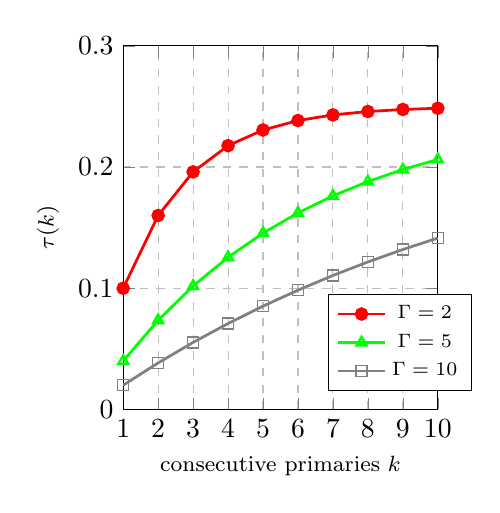
\begin{tikzpicture}
\begin{axis}[
%xmode=log,
   xlabel={consecutive primaries $k$},
   ylabel={$\tau(k)$},
    %ylabel={$\phi(x)$},
    xmin=1, xmax=10, 
    ymin=0, ymax=0.3,
    xtick={1,2,3,4,5,6,7,8,9,10},
    %xticklabels={1K, 2K, 5K, 10K, 20K,50K},
    ytick={0,0.1,0.2,0.3},
    legend pos=north west,
    ymajorgrids=true,
    grid style=dashed,
    height = 6.2cm,
    width = 0.46*\textwidth,
 %   line width=1.6pt,
%]
                legend style={at={(0.65,0.05)},anchor=south west,font=\scriptsize},
                label style={font=\footnotesize}, grid=both];
            %\addplot [black,mark=x] table [x={chi}, y={cooperative}] {\resfirsta};
        \addplot[% only marks, mark=square,  black,mark=
   color=red,mark=*,scale=10, line width=1pt,mark options={line width=0.9pt,draw=red,fill=red}]
    coordinates {
(1, 0.09999999999999998) (2, 0.15999999999999998) (3, 0.19599999999999995) (4, 0.21759999999999996) (5, 0.23055999999999996) (6, 0.23833599999999994) (7, 0.24300159999999996) (8, 0.24580095999999996) (9, 0.24748057599999995) (10, 0.24848834559999994)
    };
    \addlegendentry{$\Gamma = 2$};
    \addplot[% only marks, mark=square,  black,mark=
   color=green,mark=triangle,%dotted, 
   scale=10, line width=1pt,mark options={line width=0.9pt,draw=green,fill=green}]
    coordinates {
  (1, 0.04) (2, 0.07360000000000001) (3, 0.101824) (4, 0.12553215999999998) (5, 0.1454470144) (6, 0.162175492096) (7, 0.17622741336064) (8, 0.18803102722293757) (9, 0.19794606286726754) (10, 0.20627469280850474)
    };
    \addlegendentry{$\Gamma = 5$};
\addplot[% only marks, mark=square,
   color=gray,mark=square,scale=10, line width=1pt,mark options={line width=0.5pt,draw=gray,fill=gray}]
    coordinates {
(1, 0.019999999999999987) (2, 0.03839999999999998) (3, 0.055327999999999974) (4, 0.07090175999999997) (5, 0.08522961919999995) (6, 0.09841124966399994) (7, 0.11053834969087992) (8, 0.12169528171560953) (9, 0.13195965917836075) (10, 0.1414028864440919)
    };
    \addlegendentry{$\Gamma = 10$};
\end{axis}
\end{tikzpicture}
\label{fig_tau_beta08}} 
\subfigure[$\beta=0.9$] {
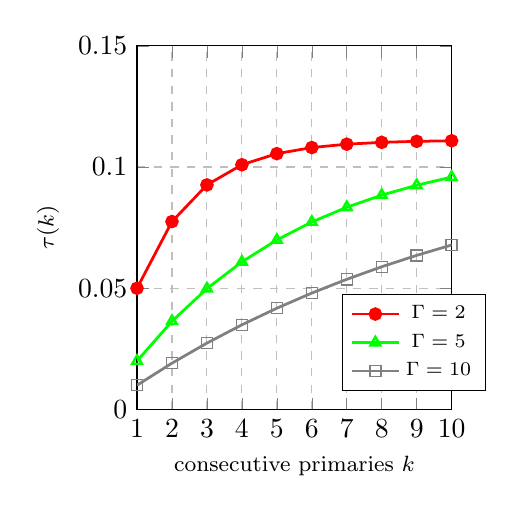
\begin{tikzpicture}
\begin{axis}[
%xmode=log,
   xlabel={consecutive primaries $k$},
   ylabel={$\tau(k)$},
    %ylabel={$\phi(x)$},
    xmin=1, xmax=10, 
    ymin=0, ymax=0.15,
    xtick={1,2,3,4,5,6,7,8,9,10},
    %xticklabels={1K, 2K, 5K, 10K, 20K,50K},
    ytick={0,0.05,0.1,0.15},
    yticklabels={0,0.05,0.1,0.15},
    legend pos=north west,
    ymajorgrids=true,
    grid style=dashed,
    height = 6.2cm,
    width = 0.46*\textwidth,
 %   line width=1.6pt,
%]
                legend style={at={(0.65,0.05)},anchor=south west,font=\scriptsize},
                label style={font=\footnotesize}, grid=both];
            %\addplot [black,mark=x] table [x={chi}, y={cooperative}] {\resfirsta};
        \addplot[% only marks, mark=square,  black,mark=
   color=red,mark=*,scale=10, line width=1pt,mark options={line width=0.9pt,draw=red,fill=red}]
    coordinates {
(1, 0.04999999999999998) (2, 0.07749999999999997) (3, 0.09262499999999997) (4, 0.10094374999999997) (5, 0.10551906249999997) (6, 0.10803548437499998) (7, 0.10941951640624997) (8, 0.11018073402343746) (9, 0.11059940371289059) (10, 0.11082967204208981)
    };
    \addlegendentry{$\Gamma = 2$};
    \addplot[% only marks, mark=square,  black,mark=
   color=green,mark=triangle,%dotted, 
   scale=10, line width=1pt,mark options={line width=0.9pt,draw=green,fill=green}]
    coordinates {
(1, 0.019999999999999987) (2, 0.036399999999999974) (3, 0.049847999999999976) (4, 0.06087535999999996) (5, 0.06991779519999995) (6, 0.07733259206399996) (7, 0.08341272549247995) (8, 0.08839843490383356) (9, 0.09248671662114352) (10, 0.09583910762933767)
    };
    \addlegendentry{$\Gamma = 5$};
\addplot[% only marks, mark=square,
   color=gray,mark=square,scale=10, line width=1pt,mark options={line width=0.5pt,draw=gray,fill=gray}]
    coordinates {
(1, 0.009999999999999993) (2, 0.01909999999999999) (3, 0.027380999999999982) (4, 0.034916709999999976) (5, 0.04177420609999997) (6, 0.04801452755099997) (7, 0.05369322007140997) (8, 0.058860830264983066) (9, 0.06356335554113458) (10, 0.06784265354243246)
    };
    \addlegendentry{$\Gamma = 10$};
\end{axis}
\end{tikzpicture}
\label{fig_tau_beta09}} 
\caption{The value of $\tau(k)$ calculated for different values of $\Gamma$ and $k$}
\label{fig:tau_vs_k_beta}
\end{figure}



 


From the table one can easily conclude that within a very small number of consecutive correct terms, the global Epool distribution recovers almost completely (typically already four terms are enough). Moreover, the damage consecutive Byzantine primaries can cause is bounded by a small fraction. Further notice that the probability for consecutive Byzantine primaries is low: for $k=5$ and $\frac{f}{n}=\frac{1}{3}$, this probability is $\frac{1}{243}$ (and of course much lower for smaller $\frac{f}{n}$). While we leave a more complete probabilistic analysis of the possible sequences for Byzantine/correct primaries to future work, the intuition illustrated in the above table is already satisfactory. We can derive from it that at all times, at least an $\eta$ fraction of the $GEP$ distribution corresponds to $\MC{I}$. Put differently, at all times we have $\norm{\MBG^r-\MBI}\leq 1-\eta$. In view of the table, $\eta$ should be considered as being quite large (say, larger than $0.7$).

%FUTURE WORK
%
%\begin{corollary}
%	\red{waiting time fairness?}
%\end{corollary}

\textbf{Chain fairness.}
We finish with one final property of representation fairness, which states that the chain distribution is very close to the issuance distribution. Denote by $\delta_f^r$ the number of faulty terms up to term $r$ (In expectancy, $\delta_f^r \leq \frac{f}{n}\cdot r$). By a slight abuse of notation we denote by $\MC{I}^r$ the set of all $etx$s issued \textbf{up to} term $r$. We also denote by $\MC{H}^r$ the set of hidden $etx$s which were appended to the blockchain by term $r$. Observe that $\MC{H}^r=\MC{C}^r\setminus \MC{I}^r$. We start with the following lemma:
\begin{lemma} \label{lemma:hidden}
	$|\MC{H}^r|\leq \delta_f^r \cdot (1-\beta)\cdot b$.
\end{lemma}
\begin{proof}
For a faulty term $s$ we denote by $\widetilde{EB^s}$ the Eblock committed on term $s$. For a correct term, we denote the committed Eblock by $EB^s$. It holds that:
\begin{align}
\MC{C}^r\setminus \MC{I}^r &= \left(\bigcup_{s\leq r \text{ faulty term}}\widetilde{EB^s} \bigcup_{s\leq r \text{ correct term}} EB^s\right)\mathbin{\big\backslash} \MC{I}^r \nonumber \\
&= \bigcup_{s\leq r \text{ faulty term}} \left (\widetilde{EB^s} \mathbin{\big\backslash} \MC{I}^r \right ) \bigcup_{s\leq r \text{ correct term}} \left (EB^s \mathbin{\big\backslash} \MC{I}^r \right )\label{eq:rep_e}
\end{align}
For the correct terms, the $etx$s in $EB^s$ are assumed in our model to be a precise representation of $\MBG^s$, and in any case do not include any hidden $etx$s. For a faulty term $s$ we know that $|\widetilde{EB^s}\cap EB^s_i|>\beta\cdot b$ for some correct node $i$. Since $i$ constructs a valid Eblock, $EB_i\subseteq GEP^s$ and these $etx$s are not hidden. In particular, we conclude that $|\widetilde{EB^s}\setminus \MC{I}^s|\leq (1-\beta)\cdot b$. We thus have 
$$|\MC{H}^r| \leq \delta_f^r \cdot (1-\beta)\cdot b$$  for all $r$.
\end{proof}
We are now ready to state and prove our main result regarding chain fairness.
\begin{claim}[Chain fairness]
In \nameNS, under the model assumptions presented above, for all $r$ it holds that: $\norm{\MBC^r-\MBI} \leq 2\cdot\big(\frac{(1-\eta)\cdot\Gamma}{r}+\frac{\delta_f^r\cdot (1-\beta)}{r}\big)$.
\end{claim}
\noindent 

We make a couple of remarks regarding the bound in the above claim. The first component accounts for the distortion caused by biased sampling, while the second is due to the absolute number of hidden $etx$s, computed in the above lemma. Now, recall that in the eyes of a third party $etx$s of two correct nodes are indistinguishable. We are thus led to assume that the difference of $2\cdot\big(\frac{(1-\eta)\cdot\Gamma}{r}+\frac{\delta_f^r\cdot (1-\beta)}{r}\big)$ is in fact shared among all $n-f$ correct nodes equally, yielding a much smaller bound on the actual deviation of each correct node from its true representation. Finally we note that in our proof we allow Byzantine primaries to use a $(1-\beta)$-fraction of hidden $etx$s, \textbf{in addition} to a $(1-\beta)$-fraction of biased sampling. This multiplies the actual damage Byzantine primaries can cause (i.e., the bound if the claim) by a factor of $2$. We do this for the sake of brevity, and it can easily be corrected by adding another variable to model a convex combination of these attacks rather than allowing both of them simultaneously.
 
\begin{proof}
%change notation for $\MC{I}^r$

Observe that the set of appended $etx$s $\MC{C}^r$ is composed issued $etx$s, which lie in $\MC{I}^r$, and some hidden $etx$s, which were added to the blockchain by Byzantine primaries.
%\footnote{A Byzantine primary would probably forward its hidden $etx$s after including them in its $EB$, thus formally 'issuing' them. We nevertheless regard such $etx$ as though they were never issued.}
Hence $\MC{C}^r=\MC{CI}^r\cup \MC{H}^r$, where $\MC{CI}^r:=\MC{C}^r\cap \MC{I}^r$. On the other hand, $\MC{I}^r$ is composed of the $etx$s which were already appended to the blockchain, namely those which lie in $\MC{C}^r$, in addition to those which have not yet been appended - which lie in $GEP^r$. We conclude $I^r=\MC{CI}^r\cup GEP^r$. We use these decompositions to analyze the distance $\norm{\MBC^r-\MBI}$ between the distributions, by using the fact that $\MBCI^r$ is the significant factor in both $\MBI^r$ and $\MBC^r$. We then use the fact that, as our previous claim shows, the distribution of $GEP^r$ is close to $\MC{I}$. Let $\MBCI^r$ denote the distribution of $etx$s among nodes in $\MC{CI}^r$, and $\mathbf{H}^r$ the distribution of hidden $etx$s, we have the following identities:
\begin{enumerate}
	\item  $\MBC^r=\frac{1}{|\MC{C}^r|}\left(|\MC{C}I^r|\cdot \MBCI^r+|\MC{H}^r|\cdot \mathbf{H}^r\right)$.
	\item $\MBI=\frac{1}{|\MC{I}^r|}\left(|\MC{C}I^r|\cdot\MBCI^r +|GEP^r|\cdot\MBG^r\right)$. % and multiplying by $|\MC{I}^r|$ we get $\MBCI^r=\frac{|\MC{I}^r|}{|\MC{CI}^r|}\cdot\MBI-\frac{|GEP^r|}{|\MC{CI}^r|}\cdot\MBG^r$.
	.
\end{enumerate}
Plugging the second formula to the first one and canceling the $|\MC{CI}^r|$  factor, we get 
$$\MBC^r=\frac{1}{|\MC{C}^r|}\left(|\MC{I}^r|\cdot\MBI-|GEP^r|\cdot \MBG^r+|\MC{H}^r|\cdot \mathbf{H}^r\right).$$
By the definition of $\eta$, at all times at least an $\eta$ fraction of $\MBG^r$ is distributed according to $\MBI$. As we are doing a worst-case analysis, we assume that  $\MBG^r=\eta \cdot\MBI+(1-\eta)\cdot \MBG_B^r$  and conclude
%\begingroup\makeatletter\def\f@size{7}\check@mathfonts
 \begin{equation}\begin{split}
 \norm{\MBC^r-\MBI} & =  \left \lVert \frac{1}{|\MC{C}^r|}\big(\left(|\MC{I}^r|-\eta\cdot |GEP^r|\right)\cdot \MBI+ (1-\eta)\cdot|GEP^r|\cdot \MBG^r_B+|\MC{H}^r|\cdot \mathbf{H}^r\big)-\MBI \right \rVert \\
& \leq \frac{\Big| |\MC{I}^r|-\eta\cdot |GEP^r|-|\MC{C}^r|\Big|}{|\MC{C}^r|}\cdot \norm{\MBI}+ \frac{(1-\eta)\cdot|GEP^r|}{|\MC{C}^r|}\cdot \norm{\MBG_B^r}+\frac{|\MC{H}^r|}{|\MC{C}^r|}\cdot \norm{\mathbf{H}^r}. 
\end{split}\end{equation}
%\endgroup
As $\norm{\MBI}=\norm{\MBG^r_B}=\norm{\mathbf{H}}=1$, the above is bounded by 
$$ \frac{\bigg| |\MC{I}^r|-\eta\cdot |GEP^r|-|\MC{C}^r|\bigg|}{|\MC{C}^r|}+\frac{(1-\eta)\cdot|GEP^r|}{|\MC{C}^r|}+\frac{|\MC{H}^r|}{|\MC{C}^r|}.$$
Recall that $\MC{I}^r=(\MC{C}^r\setminus \MC{H}^r)\cup GEP^r$. Together with the fact that $\MC{H}^r\subset \MC{C}^r$ and $GEP\cap \MC{C}^r=\emptyset$, we get $|\MC{I}^r|=|\MC{C}^r|-|\MC{H}^r|+|GEP^r|$. Using this equality for the first component above yields 
$$\big| |\MC{I}^r|-\eta\cdot |GEP^r|-|\MC{C}^r|\big|=\big| |\MC{C}^r|-|\MC{H}^r|+|GEP^r|-\eta\cdot|GEP^r|-|\MC{C}^r|\big|\leq(1-\eta)\cdot |GEP^r|+|\MC{H}^r|,$$ 
and we get
$$\norm{\MBC^r-\MBI}\leq 2\frac{(1-\eta)\cdot|GEP^r|+|\MC{H}^r|}{|\MC{C}^r|}.$$
We Assume $|GEP|=\Gamma b$, and by definitions we know $|\MC{C}^r|=b\cdot r$. In addition, lemma~\ref{lemma:hidden} proves $|H^r|\leq \delta_f^r \cdot (1-\beta)\cdot b$. Adding all up results in
$$\norm{\MBC^r-\MBI}\leq 2\cdot\big(\frac{(1-\eta)\cdot\Gamma}{r}+\frac{\delta_f^r\cdot (1-\beta)}{r}\big).$$
\end{proof}


% The first thing property we wish to ensure is that $\mathbf{P}^r$ is quick to recover from distortions created by biased sampling. 

% Fix a node $i$. For brevity, we omit $i$ from the notations. We would like to show that for all $r$, $\mathbf{P}^r$ is close to $\mathbf{I}$. Notice that this question is deeply related to the question of whether $\mathbf{B}^r$ is close to $\mathbf{I}^0$, but they are not equivalent - small bias in $\mathbf{B}^r$ can a-priori accumulate over time to a significant bias in $\mathbf{P}^r$. The question is thus reduced to whether or not a $(1-\beta)$ fraction of $EB$ can have an accumulative (short term) effect, and how long can this effect last. Our result in this context is the following:
% \begin{claim}{}
%     Suppose $r_0$ is a faulty term followed by $k$ correct terms. Assume that $\mathbf{P}^{r_0}=\mathbf{I}$, which means that at term $r_0$ the Epool distribution is exactly the issuance rate. For a correct user $j$, we have  
%     $$|\mathbf{P}^{r_0}_j-\mathbf{P}^{r_0+k}_j|=|\mathbf{I}_j-\mathbf{P}^{r_0+k}_j|\leq\left(1-\beta\right)\frac{1}{\Gamma}\left(1-\frac{1}{\Gamma}\right)^k\mathbf{I}_j$$
%      That is, the difference between the 'real' distribution of $j$'s $etx$s and the distribution as seen in the Epool decreases exponentially in the number of consecutive correct terms.
% \end{claim}

% We remark that there are, of course, other scenarios to consider - particularly: 
% \begin{enumerate}
% \item $\mathbf{P}^{r_0}\ne \mathbf{I}$.
% \item During the $k$ terms after $r_0$ there is another Byzantine primary.
% \end{enumerate}
% However, we stress that the larger the initial disruption is, the 'correction' rate in correct terms would also increase. This gives intuition for the first scenario. Regarding the second scenario we note that the number of terms required for an effective recovery to the real issuance rate is rather small \red{(around 3 terms, see the examples right after the proof below)}. For this reason, we do not expect many Byzantine primaries before the distribution recovers. When such a case does occur, we can still rely on the above remark, namely that the rate of convergence back to the issuance rate is fast enough so as to prevent an accumulative disruption of the distribution $\mathbf{P}^r$. These arguments give a (informal) justification for the assumptions in the lemma.

% \begin{proof} 
% An Eblock of a faulty primary $EB$ is modelled by drawing a $\beta$ fraction of it from $\mathbf{P}^r$ and a $(1-\beta)$ fraction of sampling freely. So $EB^{r}=b\left(\beta\cdot \mathbf{P}^r + \left(1-\beta\right)\cdot \mathbf{P}_f^r\right)$, where $\mathbf{P}^r_f$ is any possible probability vector (i.e., a probability vector which can be realized in $GEP$. Suppose $\mathbf{P}^r=\mathbf{I}$, and that $r$ is a faulty term. We have 
%     $$\MBP^{r+1}=\MBP^r+\frac{1}{\Gamma b}(b\cdot \MBI-b\cdot \MBB^r)=\MBI+\frac{1}{\Gamma b}\Big(b\cdot \MBI-b\cdot\left(\beta \MBI+\left(1-\beta\right) \MBP^r_f\right)\Big)$$
%     where $b\cdot \MBI$ accounts for the issued $etx$s of the term, and $-b\cdot \MBB^r$ for the appended $etx$s of the term (i.e., for $EB^r$). Considering only the $j$'th coordinate, the worst case scenario (from $j$'s perspective), is that $(\MBP_f^r)_j=0$. In words, this simply means that the faulty component does not include any $etx$ of node $j$. We assume this is the case, as it is both the worst case and, to a large extent, the probable one \footnote{The primary is likely to use this fraction as much as it can, including others $etx$s only if it doesn't have enough $etx$s of its own}. We get $\MBP^{r+1}_j=\MBI_j+\frac{1}{\Gamma}\cdot(1-\beta)\MBI_j$ and hence $|\MBP^{r+1}_j-\MBI_j|=\frac{1-\beta}{\Gamma}\cdot \MBI_j$. 
    
%     $\frac{1-\beta}{\Gamma}$ is the 'damage' the faulty caused to node $j$. Now the correct terms start to 'stabilize' the system. As $j$'s fraction in $\MBP^{r+1}$ is now larger than it's fraction in $\MBI$, at each term there would be more of $j$'s $etx$s appended to the blockchain than $etx$s issued by $j$. In other words, for a correct term $r+k$, $\MBB^{r+k}=\MBP^{r+k}$, so we get in the general case:
%     $$\MBP^{r+k}=\MBP^{r+(k-1)}+\frac{1}{\Gamma b}(b\cdot \MBI-b\cdot \MBP^{r+(k-1)})=(1-\frac{1}{\Gamma})\MBP^{r+(k-1)}+\frac{1}{\Gamma}\MBI$$
%     This gives an inductive formula for $\MBP^{r+k}$. We can now prove that $\MBP^{r+k}_j=\left(1+\left(1-\beta\right)\frac{1}{\Gamma}\left(1-\frac{1}{\Gamma}\right)^k\right)\MBI_j$; the base case was shown above, for $k=0$, in the faulty term. Assume the formula holds for $k-1$, and by the formula for $\MBP^{r+k}_j$ we get
%     $$\MBP^{r+k}_j=\left(1-\frac{1}{\Gamma}\right)\MBP^{r+(k-1)}+\frac{1}{\Gamma }\MBI=\left(1-\frac{1}{\Gamma}\right)\Bigg(1+(1-\beta)\frac{1}{\Gamma}\left(1-\frac{1}{\Gamma}\right)^{k-1}\Bigg)\MBI_j+\frac{1}{\Gamma}\MBI_j$$
%     Rearranging, we get
%     $$\MBP^{r+k}_j=\left(1-\frac{1}{\Gamma}\right)\MBI_j+\Bigg(\left(1-\beta\right)\frac{1}{\Gamma}\left(1-\frac{1}{\Gamma}\right)^k\Bigg)\MBI_j+\frac{1}{\Gamma}\MBI_j$$
%     The $\frac{1}{\Gamma}\MBI_j$ factors cancel each other, and we are left with $\MBP^{r+k}_j=\left(1+\left(1-\beta\right)\frac{1}{\Gamma}\left(1-\frac{1}{\Gamma}\right)^k\right)\MBI_j$, completing the inductive proof. We conclude that $|\MBP^{r+k}_j-\MBI_j|\leq\left(1-\beta\right)\frac{1}{\Gamma}\left(1-\frac{1}{\Gamma}\right)^k\MBI_j$ as claimed.
% \end{proof}
% \red{MAKE THE TABLE}
% The following table gives the distance $|\MBI_j-\MBP^{r+k}_j|$ for different values of $b,\Gamma$ and $k$.
 

% \begin{corollary}
% 	\red{For all $r$, $\MBP^r=\eta \MBI+(1-\eta)\cdot\MBP_f^r$ for $\eta=***$.}
% \end{corollary}
% \begin{corollary}
% 	\red{waiting time fairness?}
% \end{corollary}

% We finish with a third property of representation fairness, which states that the chain rate is very close to the issuance rate.  Denote by $\delta_f^r$ the number of faulty terms up to term $r$.
% \begin{claim}{} 
% In Gruffalo, $\norm{\MBC^r-\MBI}_{\ell^1} \leq 2\frac{(1-\eta)\cdot\Gamma}{r}+2\cdot \delta_f^r\cdot (1-\beta)$.
% \end{claim}

% We right away make a couple of remarks. First, recall that $etx$s are encrypted. Hence, no distinction can be made between two correct nodes. We are thus led to assume that the above difference of $2\frac{(1-\gamma)\cdot\Gamma}{r}+2\cdot \delta_f^r\cdot (1-\beta)$ is in fact shared among all $\frac{n-f}{n}$ nodes, yielding a much smaller bound on the actual deviation of each node from its true representation. Second, in our proof we allow faulty primaries to use a $(1-\beta)$ fraction for hidden $etx$s, \textbf{in addition} to a $(1-\beta)$ fraction of biased sampling. This multiplies the actual harm a faulty primary can cause by a factor of $2$. We allow it for the sake of brevity, and it can easily be corrected by adding another variable to model a convex combination of these attacks rather than allowing both of them simultaneously.
 
% \begin{proof}
% By a slight abuse of notation we denote by $\MC{I}^r$ the set of all issued $etx$s up to term $r$. We also denote by $\MC{H}^r$ the set of hidden $etx$s which were appended to the blockchain by term $r$, and observe that $\MC{H}^r=\MC{C}^r-\MC{I}^r$. A term in which the primary that got its Eblock committed was faulty is called a `faulty term', and otherwise we call the term 'non-faulty'. We start with the following lemma:
% \begin{lemma}
% 	$|\MC{H}^r|\leq \delta_f^r\cdot r \cdot (1-\beta)\cdot b$.
% \end{lemma}
% \begin{proof}
% For a faulty term $t$ we denote by $\widetilde{EB^t}$ the Eblock committed on term $t$. For a non faulty term, we denote the committed Eblock by $EB^t$. It holds that:
% \begin{align}
% \MC{C}^r\setminus \MC{I}^r &= \left(\bigcup_{t\leq r \text{ faulty term}}\widetilde{EB^t} \bigcup_{t\leq r \text{ non faulty term}} EB^t\right)\mathbin{\big\backslash} \MC{I}^r \nonumber \\
% &= \bigcup_{t\leq r \text{ faulty term}} \left (\widetilde{EB^t} \mathbin{\big\backslash} \MC{I}^r \right ) \bigcup_{t\leq r \text{ non faulty term}} \left (EB^t \mathbin{\big\backslash} \MC{I}^r \right )\label{eq:rep_e}
% \end{align}
% For the non faulty terms, the $etx$s in $EB^t$ are assumed in our model to be a precise representation of $\MC{P}^r$, and in any case do not include any hidden $etx$s. For a faulty term $t$ we know that $|\widetilde{EB^t}\cap EB^t_i|>\beta\cdot b$ for some correct node $i$. Since $i$ constructs a valid Eblock, $EB_i\subset GEP^r$ and these $etx$s are not hidden. In particular, we conclude that $|\widetilde{EB^t}\setminus \MC{I}^r|\leq (1-\beta)\cdot b$. We thus have 
% $$|\MC{H}^r| \leq \delta_f^r\cdot r \cdot (1-\beta)\cdot b$$  for all $r$, as wanted.
% \end{proof}
% Observe next that the set of appended $etx$s $\MC{C}^r$ is composed of issued $etx$s, which lie in $\MC{I}^r$, and some hidden $etx$s which were added to the blockchain by faulty primaries\footnote{A faulty primary would probably forward its hidden $etx$s after including them in its $EB$, thus formally 'issuing' them. We nevertheless regard such $etx$ as though they were never issued.}. Hence $\MC{C}^r=\MC{C}I^r\cup \MC{H}^r$, where $\MC{H}^r$ is the set of all hidden $etx$s which were appended to the blockchain by term $r$, and $\MC{CI}^r:=\MC{C}^r\cap \MC{I}^r$. On the other hand, $\MC{I}^r$ is composed of the $etx$s which were already appended to the blockchain, and thus lie in $\MC{C}^r$, and those which have not yet been appended, which lie in $GEP^r$. So $I^r=\MC{CI}^r\cup GEP^r$. We use this partition to analyse the distance between the distributions $\norm{\MBC{C}^r-\MBI}$. Letting $\MBCI^r$ denote the distribution of $etx$s among nodes in $\MC{CI}^r$, and $\mathbf{H}^r$ the distribution of hidden $etx$s, we have the following identities:
% \begin{enumerate}
% 	\item  $\MBC^r=\frac{1}{|\MC{C}^r|}\left(|\MC{C}I^r|\cdot \MBCI^r+|\MC{H}^r|\cdot \mathbf{H}^r\right)$.
% 	\item $\MBI=\frac{1}{|\MC{I}^r|}\left(|\MC{C}I^r|\cdot\MBCI^r +|GEP^r|\MBP^r\right)$, and multiplying by $|\MC{I}^r|$ we get $\MBCI=\frac{|\MC{I}^r|}{|\MC{CI}^r|}\cdot\MBI-\frac{|GEP^r|}{|\MC{CI}^r|}\MBP^r$.
% 	\item $|\MC{I}^r|=|\MC{CI}^r|+|GEP^r|$, and we have $\MBI=\frac{1}{|I^r|}\left(|\MC{CI}^r|\MBI+|GEP^r|\MBI\right)$
% \end{enumerate}
% Plugging the second formula to the first one and canceling the $|\MC{C}^r|$  factor, we get 
% $$\MBC^r=\frac{1}{|\MC{C}^r|}\left(|\MC{I}^r|\cdot\MBI-|GEP^r|\MBP^r+|\MC{H}^r|\cdot \mathbf{H}^r\right)$$
% By the previous claim, at all times we have that $\MBP^r=\eta \cdot\MBI+(1-\eta)\cdot \MBP_f^r$ for some appropriate $\eta$. We conclude that 
%  \begin{align}
%  \norm{\MBC^r-\MBI} \nonumber
%  & =\norm{\frac{1}{|\MC{C}^r|}\left(\left(|I^r|-\eta\cdot |GEP^r|\right)\cdot \MBI+ (1-\eta)\cdot|GEP^r|\MBP^r_f+|\MC{H}^r|\cdot \mathbf{H}^r\right)-\MBI} \nonumber\\
%  & \leq \frac{|\MC{I}^r|-\eta\cdot |GEP^r|-|\MC{C}^r||}{|\MC{C}^r||}\norm{\MBI}+\frac{(1-\eta)\cdot|GEP^r|}{|\MC{C}^r|}\norm{\MBP_f^r}+\frac{|\MC{H}^r|}{|\MC{C}^r|}\norm{\cdot \mathbf{H}^r}\nonumber \\
% \end{align}
% As $\norm{\MBI}=\norm{\MBP^r_f}=\norm{\mathbf{H}}=1$, the above is bounded by 
% $$ \frac{|\MC{|}I^r|-\eta\cdot |GEP^r|-|\MC{C}^r||}{|\MC{C}^r|}+\frac{(1-\eta)\cdot|GEP^r|}{|\MC{C}^r|}+\frac{|\MC{H}^r|}{|\MC{C}^r|}$$
% Recall that $\MC{I}^r=(\MC{C}^r\setminus \MC{H}^r)\cup GEP^r$, and that $\MC{H}^r\subset \MC{C}^r,\ GEP\cap \MC{C}^r=\emptyset$, so we get $|\MC{I}^r|=|\MC{C}^r|-|\MC{H}^r|+|GEP^r|$. 
% $$|\MC{I}^r|-\eta\cdot |GEP^r|-|\MC{C}^r||=||\MC{C}^r|-|\MC{H}^r|+|GEP^r|-eta\cdot|GEP^r|-|\MC{C}^r||=|(1-\eta)\cdot |GEP^r|+|\MC{H}^r||$$ 
% And we eventually get 
% $$\norm{\MBC^r-\MBI}\leq 2\frac{(1-\eta)|GEP^r|+|\MC{H}^r|}{\MC{C}^r}$$
% We assume the Epool size is $\Gamma b$, and we know $|C^r|=b\cdot r$. By the above lemma, $|H^r|\leq \delta_f^r\cdot r \cdot (1-\beta)\cdot b$.  Adding all up, we get 
% $$\norm{\MBC^r-\MBI}\leq 2\cdot \frac{(1-\eta)\Gamma\cdot b+\delta_f^r\cdot r \cdot (1-\beta)\cdot b}{br}=2\frac{(1-\eta)\cdot\Gamma}{r}+2\cdot \delta_f^r\cdot (1-\beta)$$
% As wanted.
% \end{proof}


% \red{add the conclusion of the proof in words. where can it be stronger?}


% %What proofs do we have already? Start from here and build the definition accordingly.